\documentclass[titlepage]{article}
\usepackage{graphicx}
\title{Criterion A | HL Computer Science IA}
\author{IBIS Personal Code: jhh041}
\date{Nov 24, 2022}


\begin{document}
\maketitle

\tableofcontents
\pagebreak

\section{Defining the Problem}
As the world's energy systems quickly migrate to renewables in order to combat climate change, I noticed these new systems were being inadequately taught in schools. Being one of the greatest problems of our generation, furthering the education of these systems is crucial. In particular, the pace of research, development, deployment, and results in solar energy systems are particularly eye-catching: 

\vspace*{5mm}

\begin{figure}[h]
  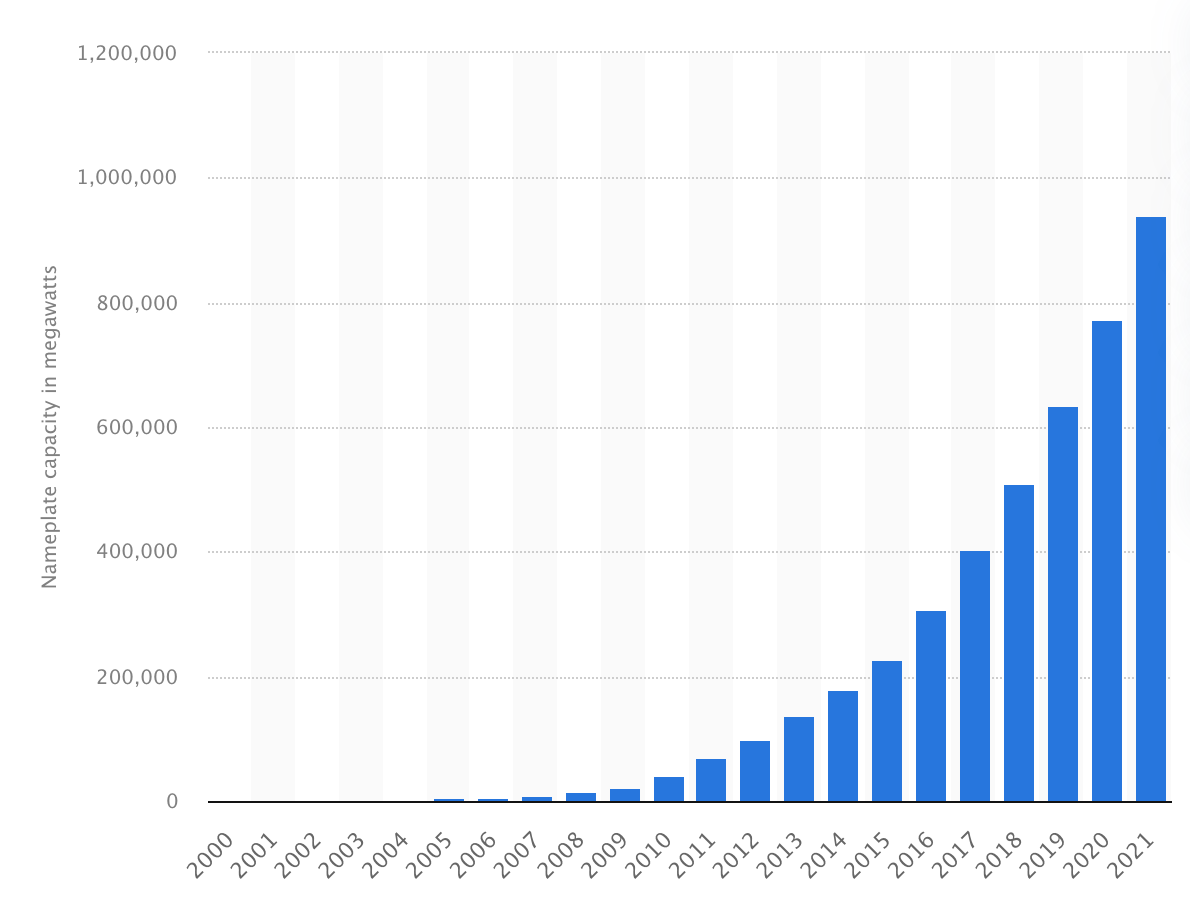
\includegraphics[width=\linewidth]{images/SCR-20221124-7e6.png}
  \caption{Cumulative sustained output of PV systems globally over time}
  \label{fig:graph}
\end{figure}

\vspace*{5mm}

\section{Proposing a Solution}
With access to an existing solar photovoltaic system, I have decided to integrate computer systems into the system with the goal of publishing live data of the system's performance to other students and the internet. This will allow students to see the performance of the system in real-time and allow them to learn about the practical applications and considerations of solar energy systems.


\end{document}
  
\documentclass[]{article}
